\section{Traitement de l'information}
%intro%
Les étapes de traitement de l'information reprennent toutes les opérations qui, d'une manière ou d'une autre, analysent et modifient le contenu original du document source ou des informations extraites. Il peut s'agir d'audit de la qualité des informations contenues dans un tableau, de la mise en place de contraintes d'intégrité, de corrections de données ou encore de regroupements de données. 
L'objectif des opérations de traitement de l'information est d'améliorer la qualité des données extraites afin qu'elle soit utilisable dans les opérations d'exploitation des données décrites dans la section suivante.

\subsection{Analyse de la qualité des données}
% définition des critères de qualité
S'il n'existe pas de consensus sur la définition même de ce que représente la qualité des données, pour autant, on peut s'accorder à dire que la qualité des données se décompose en une pluralité de critères dont la pertinence et le poids varient selon le cadre d'utilisation des informations \parencite{berti-equille_qualite_2004}. De ce constat, est né le concept \textit{fitness for use} qui dit que :
\begin{displayquote}
    \og La qualité de l'information ne renvoie jamais à la perfection de celle-ci, mais à son adéquation relative à un ensemble de besoins donnés. La tolérance à l'erreur variera en fonction des enjeux.\fg{} 
    \footfullcite[p.7]{boydens_delivrable_2007} 
\end{displayquote} 
\vspace{0,5cm}

%enjeux de la qualité dans les process automatisés
Cette qualité des données est un aspect critique dans tout processus d'automatisation. C'est particulièrement vrai lorsque plusieurs opérations automatisées se succèdent sans vérification de l'agent humain. De petites erreurs en début de processus peuvent alors se propager et prendre de l'ampleur à travers chacune des étapes suivantes. 

%exemple
Si, par exemple, à la suite d'une erreur, une escroete n'est pas détectée par l'algorithme de segmentation et n'est, de facto,  pas non plus répertoriée. De cette seule erreur, il découlerait qu'aucune connétablie située au sein de l'escroete ne serait alors répertoriée. Par extension, toutes les rentes situées dans ces connétablies seraient également non indexées et omises dans la suite du processus. Ainsi, une unique erreur peut finalement lourdement impacter les résultats obtenus en sortie du système.

%stratégie globale 
Afin d'éviter cela, des audits de la qualité des données récoltées ont été menés pendant la conception du système. En fonction des résultats rendus, les algorithmes ont été corrigés afin d'intégrer des contraintes d'intégrité (approche préventive) et des opérations de nettoyages des données(approche curative).
Dans le cas d'un système qui serait alimenté par des flux de données nouvelles, les phases d'audit devraient être intégrées au système lui-même ; on parlerait alors de \textit{gestion des processus} \parencite{berti-equille_qualite_2004}. Mais, dans le contexte qui est le nôtre, les données sont finies, plus aucune nouvelle entrée ne sera ajoutée au registre de rentes, on peut donc sortir les phases d'audit du fonctionnement du système et les cantonner au développement du système.

\subsection{Nettoyage des données}
%définition 
Le nettoyage des données est un processus d'amélioration des données qui a pour but, au travers d'une série de transformations, de normaliser les données et de détecter lorsque plusieurs enregistrements font référence à un même objet (phénomène de surcouverture) \parencite{berti-equille_qualite_2004}.

%stratégie de nettoyage %
Les stratégies pour la correction des données erronées sont aussi diverses que les causes d'où ces erreurs peuvent provenir. C'est pour cela qu'avant toute chose, il est impératif de comprendre la nature du document source et des données qu'il contient. Il faut pouvoir supposer les différents facteurs qui auraient pu altérer l'information lors de son inscription dans le document source afin de mettre en place les vérifications nécessaires pour anticiper, et le cas échéant, corriger les erreurs contenues dans le document.

%Analyse du document et des données
Dans notre cas, si nous analysons \og l'histoire \fg{} du document source, nous pouvons dire qu'il s'agit d'un document texte au format \textit{.docx} qui  a été converti au format \textit{.txt}. Or, le format \textit{.docx} prend en charge des éléments d'édition de texte qui ne le sont pas dans les fichiers \textit{.txt}. On peut donc prévoir des erreurs liées à la perte d'informations engendrée par la conversion du fichier dans un format plus basique. 
Ce document \textit{.docx} est une retranscription manuelle d'une partie du livre de G. Espinas \textit{OCRisé}.
Finalement, le livre de G. Espinas est lui-même une retranscription du registre original de Sire Jean de France. Aux erreurs provenant du changement de format du document, nous pouvons donc aussi ajouter d'éventuelles erreurs de typographie ou d'OCR \parencite{berti-equille_qualite_2004}.
Quant aux données contenues dans le document, elles sont de nature textuelle en langue picarde du XIIIe siècle. Du fait de cette particularité, les outils de nettoyage classiques sont inefficients. À l’instar de la reconnaissance d'entités nommées, il faut dans notre cas retourner à une approche plus élémentaire, basée sur une reconnaissance morphologique à l'aide d'expressions régulières. 

%doublons%
Une autre source de la perte de qualité de l'information serait la présence de doublon au sein des tableaux de données. On peut légitimement supposer qu'il n'y en a pas dans le registre original étant donné que celui-ci semble avoir été écrit de la main d'un seul homme  et que chacune des entrées du registre est classée selon un ordre topographique administratif avec un identifiant unique \parencite{espinas_les_1933}. Cependant, la possibilité que des doublons soient produits par les opérations automatisées de segmentation et de traitement n’est pas à négliger \parencite{koudoro-parfait_reconnaissance_2022}. Une vérification et une correction automatique sont donc effectuées après le remplissage de chaque tableau de données.

\subsection{Regroupement des données}
%définition %add ref
Le regroupement des données, appelé aussi \textit{clustering}, entre dans les stratégies courantes de détection et nettoyage des doublons. Elle fait donc, par définition, partie des opérations de nettoyage des données. Comme son nom l'indique, le regroupement de données va regrouper et fusionner les enregistrements d'un tableau de données qui partagent de fortes similitudes entre eux, et référençant un objet identique. 

% contexte
S'il est assez peu probable qu'il y ait des doublons au sein des rentes pour les raisons déjà énoncées, pour autant, il y en a parmi les entités nommées recensées. Ces doublons, dans ce cas précis, ne proviennent pas de négligence dans l'enregistrement des données, ou d'erreurs  produites par des processus automatisés, mais par des particularités liées au contexte historique.
En effet, dans la langue du picard médiéval, les anthroponymes peuvent subir de nombreuses variations de graphies ; un phénomène qui touche autant les noms de baptême que les patronymes. S. De Valeriola cite quatre raisons majeures à cela dans ses travaux.

%cause de la multiplicité des forme d'un anthroponymes 
Tout d'abord, les noms de baptême peuvent être déclinés en fonction de s'il est au cas sujet ou au cas régime\parencite{de_valeriola_lordinateur_2021}. Le cas sujet et le cas régime sont des cas grammaticaux hérités du latin qui, aujourd'hui, ont disparu en tant que tels dans la langue française actuelle. \parencite{kalm_roland_2009}.
Cette déclinaison se manifeste par l'ajout d'une \textit{marque casuelle} \og -s \fg{} au prénom. Ainsi, \og Joséphé \fg{} peut devenir \og Joséphés \fg{} si celui-ci est sujet. Toutefois, la présence de la marque n'est pas systématique dans les noms de personnes \parencite{mazziotta_marquage_2014}.
Ensuite, certains patronymes provenant de noms de métier ou de qualificatifs peuvent être dérivés au féminin lorsqu'ils sont portés par des femmes. On retrouve par exemple dans le registre un Druion Le Maçon, une Margritain Le Maçonnesse et  une Alis Le Maçone qui devaient probablement venir de la même famille bien que leur patronyme ne soit pas exactement identique. Également, la région n'étant pas exclusivement francophone, certains patronymes sont traduits, tantôt en picard, tantôt en flamand. Finalement, on retrouve de petites variations graphiques, sans doute dues à une certaine proximité phonétique \parencite{de_valeriola_lordinateur_2021}.

%méthode calcul de distance
La stratégie adoptée pour identifier les différentes variantes graphiques que peut prendre un même anthroponyme s'inspire, une nouvelle fois, grandement d'un article de S. De Valeriola, dans lequel il cherche à regrouper les différentes graphies de patronymes des protagonistes et témoins au sein d'actes urbains des villes du nord de la France et de Flandre, de manière semi-automatisée \parencite{de_valeriola_lordinateur_2021}.

Une fois l'ensemble des anthroponymes recensé dans une liste, la proximité morphologique entre chaque élément est calculée. Cette proximité morphologique entre deux anthroponymes est calculée selon le concept de \textit{distance d'édition}\footnote{Appelée aussi distance \textit{Levensthein}}. 
La distance d'édition entre deux chaînes de caractères est représentée par un score calculé en fonction du nombre d'opérations d'édition (suppression d'un caractère, insertion d'un caractère, substitution d'un caractère) nécessaires pour transformer une chaîne en l'autre. Il existe une multitude de distances différentes, reprenant la même idée, mais présentant chacune de légères spécificités. 
Dans notre cas, c'est la distance \textit{Damerau Levenshtein} qui a été retenue, car elle rajoute aux autres l'opération de transposition de deux caractères adjacents qui par la distance \textit{Levenshtein} était considérée comme deux opérations distinctes. 
À cette distance \textit{Damerau Levenshtein}, quelques modifications sur la pondération des différentes opérations ont été appliquées afin d'être plus juste quant aux spécificités de la langue picarde médiévale \parencite{de_valeriola_lordinateur_2021}.

%matrice 
Lorsque ces distances sont calculées, elles peuvent alors être représentées sous la forme d'une matrice. Cependant, la quantité de données  est telle qu'il est impossible de regrouper les anthroponymes sur seule base de ce tableau (avec 798 anthroponymes recensés, il est question de 636804 combinaisons). Il est par conséquent nécessaire d'automatiser le processus de regroupement en définissant  un seuil de distance qui détermine quels  anthroponymes doivent être rassemblés dans le même groupe. 

% choix de la distance seuil
Le choix de cette distance de seuil est une question particulièrement délicate et complexe qui a un impact  direct sur les résultats obtenus lors de l'exploitation des données. Si la distance seuil est trop haute, des anthroponymes risquent d'être intégrés à des groupes rassemblant des anthroponymes faisant référence à un autre personnage. Les résultats seront alors parasités par du \textit{bruit}. Ce bruit se concrétise par la fusion de sommets lors de la modélisation des graphes, ce qui créer de faux liens de mitoyenneté et déplacera également les sommets voisins, avec le risque d'une réaction en chaîne.
Au contraire, si la distance seuil est trop basse, certaines formes d'un anthroponyme risquent de ne pas être groupées avec les autres formes de variantes qui faisaient référence au même personnage. C'est du \textit{silence} qui est récolté dans ce cas. Il apparaît alors l'action inverse : au lieu que de multiples entités soient modélisées en un seul sommet, une entité unique se voit être modélisée en plusieurs sommets. Si le silence peut être relativement moins grave que le bruit dans notre contexte, dans le sens où il ne provoque pas de réactions en chaîne, il crée aussi des erreurs dans la modélisation des graphes. Il faut donc le réduire au possible.

%choix de la méthode 
Sur base du principe de calcul de distance précédemment évoqué, et au-delà du choix de la distance de seuil, il existe différentes méthodes d'application. On peut décider de calculer la distance sur l'anthroponyme entier (nom de baptême et patronyme, ensemble, considéré comme une seule chaîne de caractère) ou sur les noms de baptême  et patronymes, chacun traité séparément, dans deux matrices différentes. En plus de cela, il est encore possible de modifier la pondération des éléments du  calcul des distances, à l'instar des modifications déjà apportées par S. De Valeriola.

%ce qui a été décidé
En définitive, il a été décidé de calculer la distance sur l'entièreté de l'anthroponyme avec  une modification du poids de l'opération de substitution dans le calcul et de définir la distance de seuil à 3. 
Ces choix ont été déterminés par une série de tests destinés à observer la quantité de bruit récupérée avec les différentes méthodes. Ceux-ci seront plus amplement détaillés dans le chapitre \textit{Résultats}.

%remplacement dans le dataframe
Lorsque toute les variants graphiques de chaque anthroponyme sont recensés dans une liste par l'algorithme, cette dernière est alors vérifiée par l'agent humain. Si des erreurs sont remarquées au sein de la liste des groupes, en l'absence de solution de correction automatique, celle-ci est corrigée manuellement.

La liste vérifiée, toutes les section de rentes du tableau de données principale sont parcourues, et chaque fois qu'une forme variante d'un anthroponymes, qui a été listée, est détectée, celle-ci est un remplacée par une forme généralisée de l'anthroponyme. 

\begin{figure} % insère une figure ici (h = "here")
    \centering
    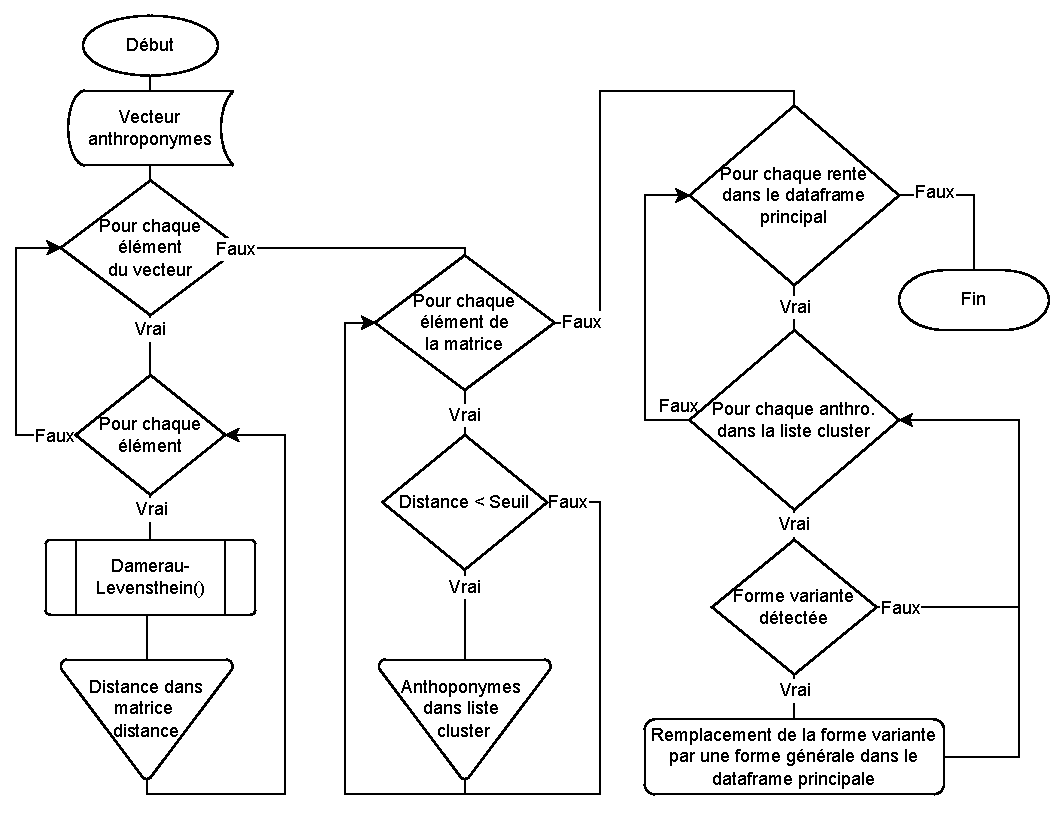
\includegraphics[scale=0.75]{2.Methods/Img/clustering.drawio.pdf} 
    \caption{Organigramme de l'algorithme de regroupement des anthroponymes}
    \label{schemaClustering}
\end{figure}


